\documentclass[11pt]{article}
\usepackage[margin=1in]{geometry}
\usepackage{amsmath,amssymb,amsthm}
\usepackage{graphicx,float}
\usepackage{lmodern}
\usepackage[T1]{fontenc}
\usepackage{xcolor,framed,booktabs,listings,microtype}
\usepackage[colorlinks=true,linkcolor=blue!60!black,urlcolor=blue!60!black]{hyperref}

\definecolor{shadecolor}{RGB}{240,244,250}
\definecolor{codebg}{RGB}{248,248,248}
\lstset{language=Python,basicstyle=\ttfamily\small,backgroundcolor=\color{codebg},
  keywordstyle=\color{blue!70!black},commentstyle=\color{green!45!black},stringstyle=\color{orange!80!black},
  frame=single,rulecolor=\color{gray!40},breaklines=true,showstringspaces=false,columns=fullflexible}

\newcommand{\R}{\mathbb{R}}
\newcommand{\norm}[1]{\left\lVert #1 \right\rVert}
\newcommand{\T}{^{\mathsf T}}
\newcommand{\lam}{\lambda}
\newcommand{\answer}[1]{\begin{shaded}\noindent\textbf{Answer.} #1\end{shaded}}

\title{Optimization --- Homework 1 \\ \large Solutions}
\author{Mitchel Carson}
\date{\today}

\begin{document}
\maketitle

\noindent\textit{Notation.} Throughout, $\norm{\cdot}$ denotes the Euclidean norm $\norm{x}_2=\sqrt{x\T x}$. A convex combination of $x,y$ means $\lam x+(1-\lam)y$ with $\lam\in[0,1]$. A set $C$ is convex if it contains every convex combination of any two of its points; a function $f$ is convex if $f(\lam x+(1-\lam)y)\le \lam f(x)+(1-\lam)f(y)$ for all $x,y$ in its (convex) domain.

%======================================================================
\section*{Problem 1. Convex Sets, Convex Functions, Preservation of Convexity}

\subsection*{(a) The intersection of convex sets is convex}

\begin{proof}
Let $C_1,C_2\subseteq\R^n$ be convex and let $C=C_1\cap C_2$. Take any $x,y\in C$ and any $\lam\in[0,1]$. Since $x,y\in C$, in particular $x,y\in C_1$; because $C_1$ is convex, $\lam x+(1-\lam)y\in C_1$. By the same argument applied to $C_2$, $\lam x+(1-\lam)y\in C_2$. A point lying in both $C_1$ and $C_2$ lies in their intersection, so $\lam x+(1-\lam)y\in C_1\cap C_2=C$. Because $x,y\in C$ and $\lam\in[0,1]$ were arbitrary, $C$ is convex.
\end{proof}

\answer{$C_1\cap C_2$ is convex. Nothing in the argument used that there are only two sets: if $\{C_\alpha\}_{\alpha\in\mathcal A}$ is \emph{any} family of convex sets (finite, countable, or uncountable), then $\bigcap_{\alpha}C_\alpha$ is convex, because a convex combination of two points of the intersection lies in every $C_\alpha$. (If the intersection is empty it is trivially convex.) This is the workhorse behind ``a polyhedron is convex'' and ``a sublevel set of a max of convex functions is convex.''}

\subsection*{(b) The union of two convex sets need not be convex}

\answer{Take $C_1=[0,1]$ and $C_2=[2,3]$ in $\R$. Both are intervals, hence convex. Their union $C_1\cup C_2=[0,1]\cup[2,3]$ contains $x=1$ and $y=2$, but the convex combination with $\lam=\tfrac12$,
\[
\tfrac12\cdot 1+\tfrac12\cdot 2=\tfrac32\notin C_1\cup C_2,
\]
so the union is not convex. Figure~\ref{fig:union} shows the same phenomenon in $\R^2$ with two disjoint disks.}

\begin{figure}[H]\centering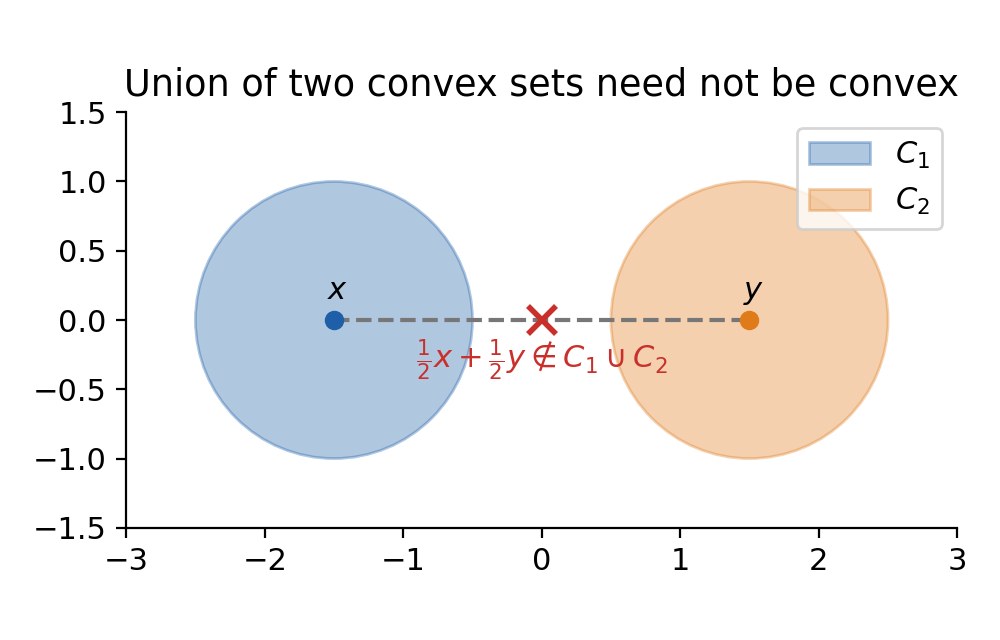
\includegraphics[width=.6\textwidth]{figures/union_not_convex.png}
\caption{Two disks are each convex, but the midpoint of $x\in C_1$ and $y\in C_2$ is in neither.}\label{fig:union}\end{figure}

\subsection*{(c) The pointwise maximum of convex functions is convex}

\begin{proof}
Let $f_1,f_2:\R^n\to\R$ be convex and define $f_{\max}(x)=\max\{f_1(x),f_2(x)\}$. Fix $x,y\in\R^n$ and $\lam\in[0,1]$, and write $z=\lam x+(1-\lam)y$. For each $i\in\{1,2\}$, convexity of $f_i$ gives
\[
f_i(z)\;\le\;\lam f_i(x)+(1-\lam)f_i(y).
\]
Now use $f_i(x)\le f_{\max}(x)$ and $f_i(y)\le f_{\max}(y)$ together with $\lam\ge0$, $1-\lam\ge0$:
\[
f_i(z)\;\le\;\lam f_i(x)+(1-\lam)f_i(y)\;\le\;\lam f_{\max}(x)+(1-\lam)f_{\max}(y).
\]
This bound holds for $i=1$ and for $i=2$, so it holds for the larger of the two:
\[
f_{\max}(z)=\max\{f_1(z),f_2(z)\}\;\le\;\lam f_{\max}(x)+(1-\lam)f_{\max}(y).
\]
Hence $f_{\max}$ is convex.
\end{proof}

\answer{$f_{\max}=\max\{f_1,f_2\}$ is convex. Two remarks:
\begin{itemize}
\item \emph{Geometric view.} $\operatorname{epi} f_{\max}=\operatorname{epi} f_1\cap\operatorname{epi} f_2$ (a point $(x,t)$ sits above the max iff it sits above both). Each epigraph is convex, so by part~(a) their intersection is convex, and a function is convex iff its epigraph is. This is the same theorem seen from the ``sets'' side.
\item \emph{Generalization.} The argument extends to finite maxima and to $f(x)=\sup_{\alpha\in\mathcal A}f_\alpha(x)$ for a nonempty family on a common convex domain. The supremum may be $+\infty$; it is convex as an extended-valued function, and its restriction to its finite domain is convex. For example, $X\mapsto\lambda_{\max}(X)$ is convex on real symmetric matrices because $\lambda_{\max}(X)=\sup_{\|u\|_2=1}u\T Xu$, a supremum of functions linear in $X$.
\end{itemize}}

\begin{figure}[H]\centering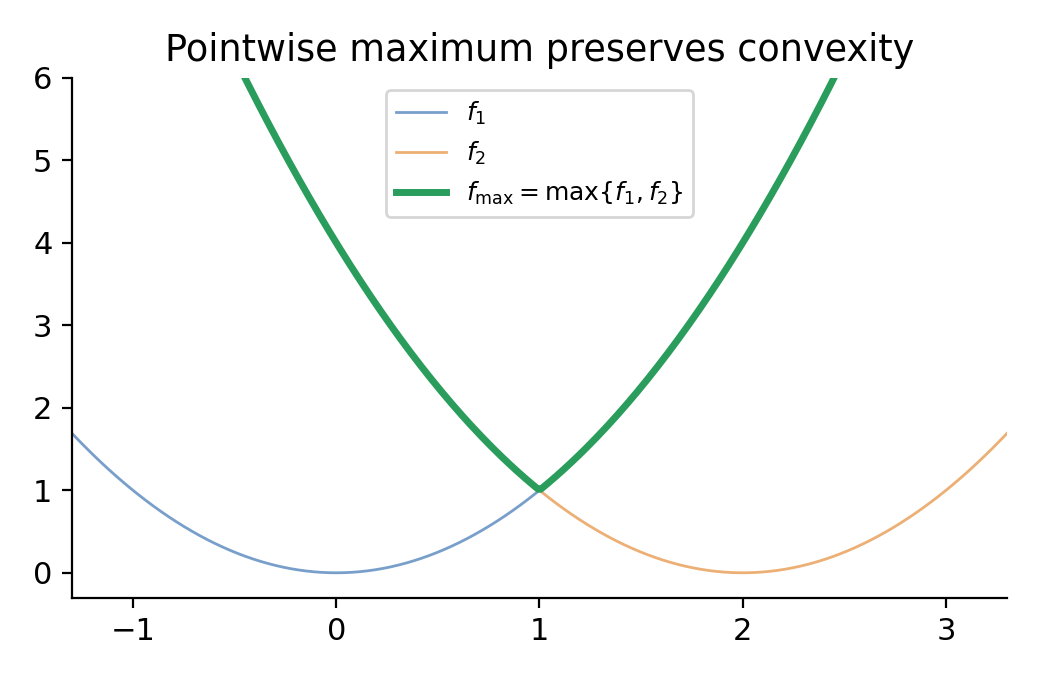
\includegraphics[width=.55\textwidth]{figures/max_convex.png}
\caption{The upper envelope of two convex parabolas is convex.}\end{figure}

%======================================================================
\section*{Problem 2. More Convex Sets, Convex Functions, Preservation of Convexity}

\subsection*{(a) The pointwise minimum of two convex functions need not be convex}

\answer{Let $f_1(x)=x^2$ and $f_2(x)=(x-2)^2$ on $\R$; both are convex. Their pointwise minimum $f_{\min}(x)=\min\{x^2,(x-2)^2\}$ satisfies
\[
f_{\min}(0)=0,\qquad f_{\min}(2)=0,\qquad f_{\min}(1)=\min\{1,1\}=1 .
\]
With $x=0$, $y=2$, $\lam=\tfrac12$ we get $f_{\min}\!\left(\tfrac12\cdot0+\tfrac12\cdot2\right)=f_{\min}(1)=1>0=\tfrac12 f_{\min}(0)+\tfrac12 f_{\min}(2)$, violating the defining inequality. So $f_{\min}$ is not convex (Figure~\ref{fig:min}). Geometrically, $\operatorname{epi} f_{\min}=\operatorname{epi}f_1\cup\operatorname{epi}f_2$ is a \emph{union} of convex sets, which (as in 1(b)) need not be convex.}

\begin{figure}[H]\centering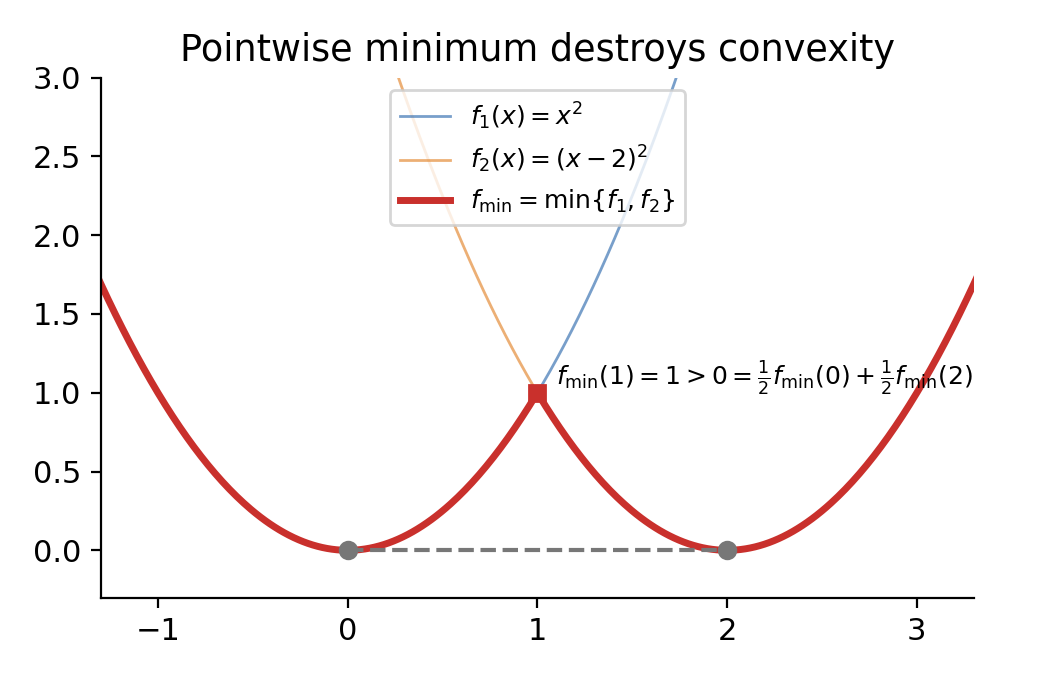
\includegraphics[width=.55\textwidth]{figures/min_not_convex.png}
\caption{The lower envelope of two parabolas has a ``bump'' at $x=1$.}\label{fig:min}\end{figure}

\subsection*{(b) Disjoint closed convex sets that cannot be strictly separated (B\&V 2.23)}

Recall the definitions from B\&V \S2.5: sets $C,D$ are \emph{separated} by the hyperplane $\{x:a\T x=b\}$ ($a\neq0$) if $a\T x\le b$ for all $x\in C$ and $a\T x\ge b$ for all $x\in D$; they are \emph{strictly separated} if $a\T x<b$ for all $x\in C$ and $a\T x>b$ for all $x\in D$.

\answer{In $\R^2$ let
\[
C_1=\{(x,y): y\le 0\},\qquad C_2=\{(x,y): x>0,\; y\ge 1/x\}.
\]
\emph{Both are convex:} $C_1$ is a half-space; $C_2$ is the epigraph of $g(x)=1/x$ restricted to $x>0$, and $g''(x)=2/x^3>0$ there, so $g$ is convex and its epigraph is convex.
\emph{Both are closed:} $C_1$ is a closed half-space. For $C_2$, if $(x_k,y_k)\in C_2$ converges to $(x,y)$, then $x\ge0$; if $x=0$ we would need $y_k\ge 1/x_k\to\infty$, impossible for a convergent sequence, so $x>0$ and by continuity $y\ge 1/x$, i.e.\ $(x,y)\in C_2$.
\emph{They are disjoint:} every point of $C_1$ has $y\le0$ and every point of $C_2$ has $y\ge1/x>0$.

\emph{They cannot be strictly separated.} Suppose, for contradiction, that $a=(a_1,a_2)\neq0$ and $b$ satisfy $a\T p<b$ for all $p\in C_1$ and $a\T q>b$ for all $q\in C_2$.
\begin{enumerate}
\item Points $(t,0)\in C_1$ for all $t\in\R$ give $a_1 t<b$ for all $t$, which forces $a_1=0$.
\item Points $(0,-t)\in C_1$ for $t\ge0$ give $-a_2 t<b$ for all $t\ge0$, which forces $a_2\ge0$; since $a\ne0$, $a_2>0$. Taking $t=0$ gives $0<b$.
\item Points $q_k=(k,1/k)\in C_2$ give $a\T q_k=a_2/k>b>0$ for every $k\ge1$. Letting $k\to\infty$ yields $0\ge b>0$, a contradiction.
\end{enumerate}
Hence no strictly separating hyperplane exists. (The unique \emph{non-strict} separating line is $y=0$, which touches $C_1$ and is approached by $C_2$ asymptotically; see Figure~\ref{fig:sep}.) Here the half-plane forces $b>0$, while the sequence $(k,1/k)$ forces $b\le0$. Although these sets also have distance zero, zero distance alone does not rule out strict separation as defined above. If one of two disjoint closed convex sets is compact, their distance is positive and strict separation is guaranteed (B\&V \S2.5.1).}

\begin{figure}[H]\centering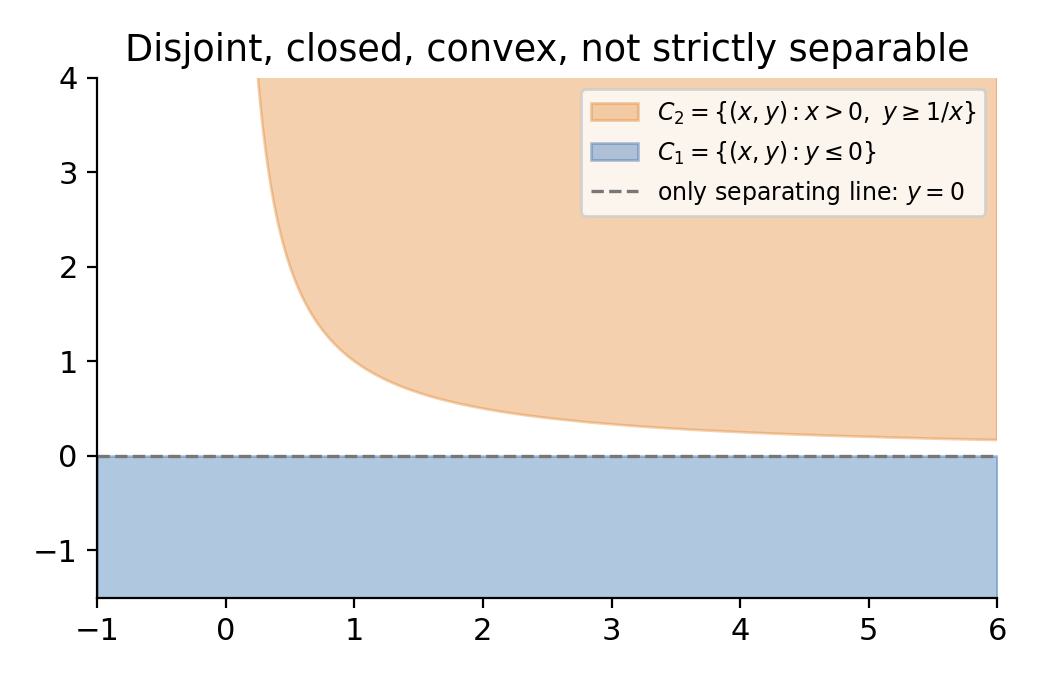
\includegraphics[width=.6\textwidth]{figures/no_strict_separation.png}
\caption{A half-plane and the region above a hyperbola: disjoint, closed, convex, but with zero distance between them.}\label{fig:sep}\end{figure}

\subsection*{(c) Sublevel sets of convex functions are convex; the converse fails}

\begin{proof}[Proof that sublevel sets are convex]
Let $f$ be convex and $c\in\R$; let $L_c=\{x:f(x)\le c\}$. Take $x,y\in L_c$ and $\lam\in[0,1]$. Then
\[
f(\lam x+(1-\lam)y)\;\le\;\lam f(x)+(1-\lam)f(y)\;\le\;\lam c+(1-\lam)c\;=\;c,
\]
where the first inequality is convexity of $f$ and the second uses $f(x)\le c$, $f(y)\le c$ with nonnegative weights. Thus $\lam x+(1-\lam)y\in L_c$, so $L_c$ is convex. (If $L_c=\emptyset$ it is convex vacuously.)
\end{proof}

\answer{\textbf{Converse is false.} Consider the univariate function $f(x)=\sqrt{|x|}$ (Figure~\ref{fig:quasi}).

\emph{All sublevel sets are convex:} for $c<0$, $L_c=\emptyset$; for $c\ge0$, $\sqrt{|x|}\le c\iff |x|\le c^2\iff x\in[-c^2,c^2]$, an interval, hence convex.

\emph{$f$ is not convex:} take $x=0$, $y=4$, $\lam=\tfrac12$. Then
\[
f\!\left(\tfrac12\cdot0+\tfrac12\cdot4\right)=f(2)=\sqrt2\approx1.414\;>\;1=\tfrac12 f(0)+\tfrac12 f(4).
\]
So the chord from $(0,0)$ to $(4,2)$ lies \emph{below} the graph, contradicting convexity.

An even simpler example is $f(x)=x^3$: every sublevel set is $L_c=(-\infty,c^{1/3}]$, an interval, yet $f''(x)=6x<0$ for $x<0$, so $f$ is not convex. In general \emph{any} monotone function of one variable has convex sublevel sets. Functions with all sublevel sets convex are called \emph{quasiconvex}; convexity is strictly stronger than quasiconvexity.}

\begin{figure}[H]\centering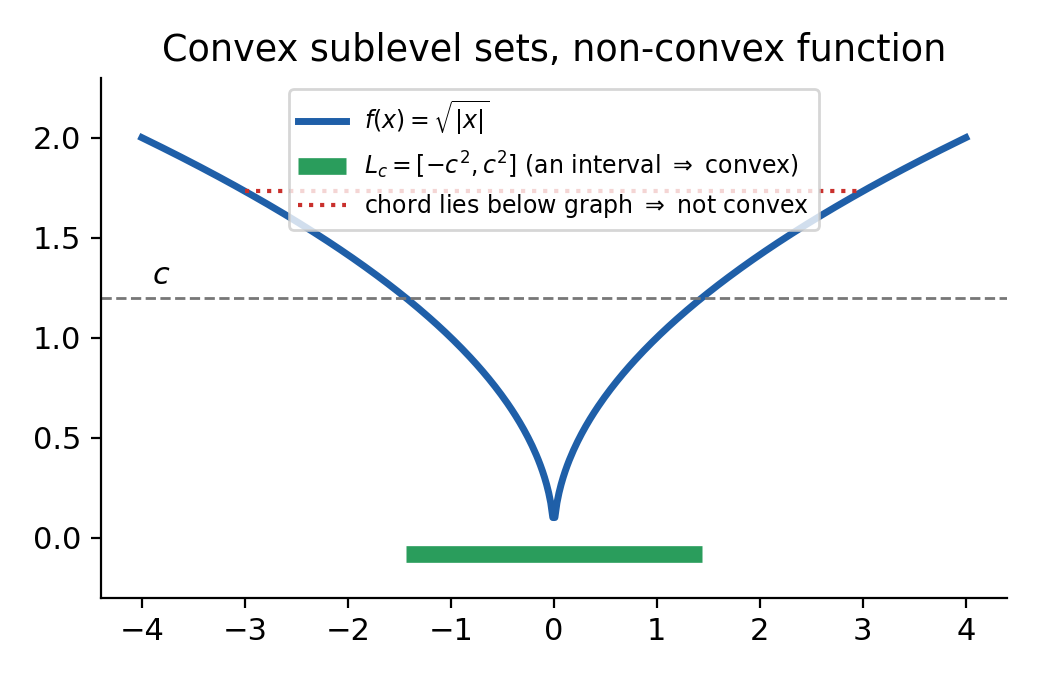
\includegraphics[width=.6\textwidth]{figures/quasiconvex.png}
\caption{$f(x)=\sqrt{|x|}$: each sublevel set is an interval, but a chord can dip below the graph.}\label{fig:quasi}\end{figure}

%======================================================================
\section*{Problem 3. Points closer to $v_1$ than to $v_2$ form a half-space}

\subsection*{Two dimensions: the picture}
With $v_1=(-1,0)$ and $v_2=(1,0)$, the set of points at least as close to $v_1$ as to $v_2$ is the closed left half-plane $\{(x_1,x_2):x_1\le0\}$, bounded by the perpendicular bisector of the segment $v_1v_2$ (the $x_2$-axis). Figure~\ref{fig:vor} shades this region.

\begin{figure}[H]\centering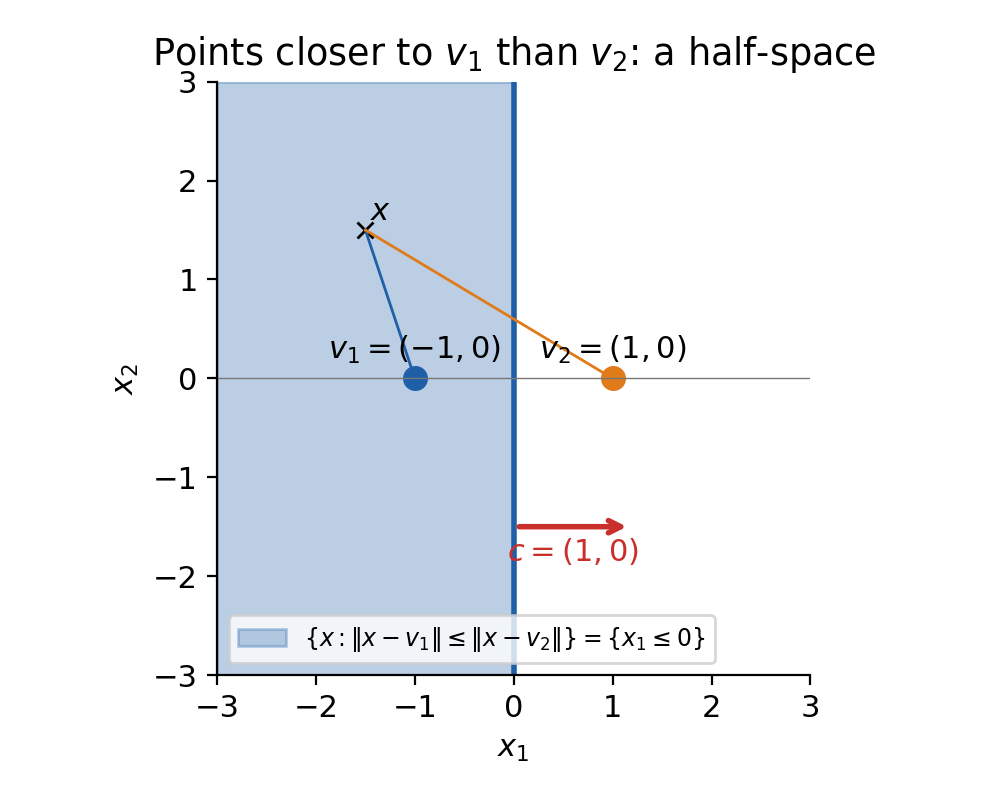
\includegraphics[width=.5\textwidth]{figures/halfspace_voronoi.png}
\caption{The shaded half-plane is $\{x:\|x-v_1\|\le\|x-v_2\|\}$; its boundary is the perpendicular bisector of $v_1v_2$.}\label{fig:vor}\end{figure}

\subsection*{Two dimensions: finding $c$ and $d$}
Since both sides are nonnegative, $\|x-v_1\|\le\|x-v_2\|\iff\|x-v_1\|^2\le\|x-v_2\|^2$. Expanding with $x=(x_1,x_2)$:
\[
(x_1+1)^2+x_2^2\;\le\;(x_1-1)^2+x_2^2
\;\iff\; 2x_1+1\le-2x_1+1
\;\iff\; 4x_1\le0
\;\iff\; x_1\le 0 .
\]
\answer{$c=(c_1,c_2)=(4,0)$ and $d=0$ describe the region as $\{(x_1,x_2):4x_1+0\cdot x_2\le0\}$. Any positive rescaling gives the same half-space, so the cleaner choice $c=(1,0)$, $d=0$ (i.e.\ $x_1\le0$) is equally valid. The normal vector $c$ points from $v_1$ toward $v_2$, i.e.\ \emph{away} from the half-space.}

\subsection*{General $v_1,v_2\in\R^n$}
\begin{proof}
For any $x\in\R^n$, expand both squared distances:
\begin{align*}
\|x-v_1\|^2 &= \|x\|^2-2v_1\T x+\|v_1\|^2,\\
\|x-v_2\|^2 &= \|x\|^2-2v_2\T x+\|v_2\|^2.
\end{align*}
Therefore
\[
\|x-v_1\|^2\le\|x-v_2\|^2
\iff -2v_1\T x+\|v_1\|^2\le-2v_2\T x+\|v_2\|^2
\iff 2(v_2-v_1)\T x\le\|v_2\|^2-\|v_1\|^2 .
\]
The quadratic term $\|x\|^2$ cancels, which is exactly why the boundary is flat rather than curved.
\end{proof}

\answer{\[
\boxed{\;c=2(v_2-v_1),\qquad d=\|v_2\|^2-\|v_1\|^2\;}
\qquad\text{so}\qquad
\{x:\|x-v_1\|_2\le\|x-v_2\|_2\}=\{x:c\T x\le d\}.
\]
When $v_1\ne v_2$ we have $c\ne0$, so this is a genuine half-space, hence convex. (If $v_1=v_2$ then $c=0,d=0$ and the set is all of $\R^n$, still convex.) For the 2-D instance, $c=2\big((1,0)-(-1,0)\big)=(4,0)$ and $d=1-1=0$, matching the previous part.

\emph{Geometric check.} The boundary hyperplane $\{x:c\T x=d\}$ passes through the midpoint $m=\tfrac12(v_1+v_2)$, because
$c\T m=(v_2-v_1)\T(v_1+v_2)=\|v_2\|^2-\|v_1\|^2=d$, and its normal $c\parallel v_2-v_1$ is the direction of the segment. It is therefore the perpendicular bisector of $v_1v_2$. Intersecting such half-spaces over several points $v_2,v_3,\dots$ gives the \emph{Voronoi cell} of $v_1$, which is convex by Problem~1(a).}

\paragraph{Numerical sanity check.} The script below draws random $v_1,v_2\in\R^5$ and $10^5$ random test points, and confirms that the distance test and the half-space test agree at every point (output in Appendix~\ref{app:code}).

%======================================================================
\section*{Problem 4 (optional). $\{x:\|Ax+b\|_2\le c\T x+d\}$ is convex}

Let $S=\{x\in\R^n:\|Ax+b\|_2\le c\T x+d\}$ with $A\in\R^{m\times n}$, $b\in\R^m$, $c\in\R^n$, $d\in\R$.

\begin{proof}[Direct proof]
Let $x,y\in S$, $\lam\in[0,1]$, and $z=\lam x+(1-\lam)y$. Because $x\mapsto Ax+b$ is affine, $Az+b=\lam(Ax+b)+(1-\lam)(Ay+b)$. Using the triangle inequality and absolute homogeneity of the norm,
\[
\|Az+b\|
\le \lam\|Ax+b\|+(1-\lam)\|Ay+b\|
\le \lam(c\T x+d)+(1-\lam)(c\T y+d)
= c\T z+d,
\]
where the second inequality uses $x,y\in S$ and $\lam,1-\lam\ge0$, and the last equality is again affinity of $x\mapsto c\T x+d$. Hence $z\in S$.
\end{proof}

\answer{$S$ is convex. Such a constraint is a second-order cone constraint; its feasible set need not be a polyhedron (Figure~\ref{fig:p4}). The numerical check in Appendix~\ref{app:code} illustrates the result for one instance; the proof above establishes it for all $A,b,c,d$.}

\begin{figure}[H]\centering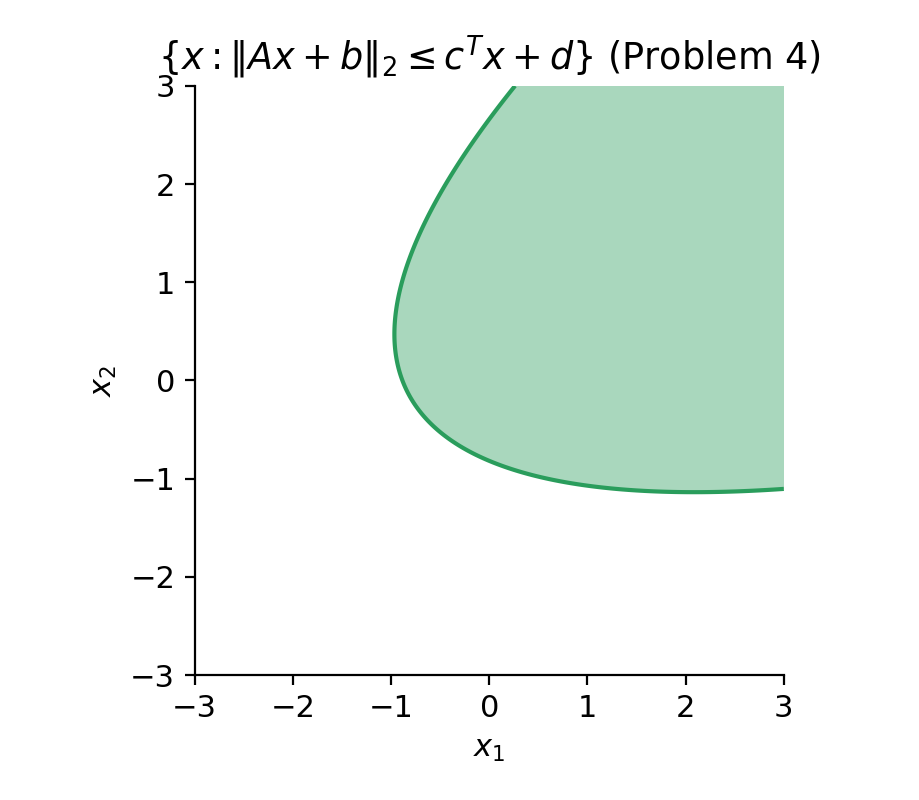
\includegraphics[width=.42\textwidth]{figures/problem4_set.png}
\caption{A two-dimensional instance of $S$ (shaded); the boundary is a conic section.}\label{fig:p4}\end{figure}

%======================================================================
\section*{Problem 5 (optional). Half-spaces and parallel hyperplanes (B\&V 2.6)}

\subsection*{(a) When does one half-space contain another?}
Let $H=\{x:a\T x\le b\}$ and $\tilde H=\{x:\tilde a\T x\le\tilde b\}$ with $a,\tilde a\ne0$.

\answer{\[
H\subseteq\tilde H\quad\Longleftrightarrow\quad \exists\,\lam>0:\ \tilde a=\lam a\ \text{ and }\ \tilde b\ge\lam b .
\]
\[
H=\tilde H\quad\Longleftrightarrow\quad \exists\,\lam>0:\ \tilde a=\lam a\ \text{ and }\ \tilde b=\lam b .
\]
In words: the normals must point in the same direction, and after matching their lengths the second threshold must be at least as large (or equal, for equality of the sets).}

\begin{proof}
($\Leftarrow$) If $\tilde a=\lam a$, $\tilde b\ge\lam b$ with $\lam>0$, and $x\in H$, then $\tilde a\T x=\lam a\T x\le\lam b\le\tilde b$, so $x\in\tilde H$.

($\Rightarrow$) Assume $H\subseteq\tilde H$. Let $x_0=\dfrac{b}{\|a\|^2}a$, which satisfies $a\T x_0=b$, so $x_0\in H$.

\emph{Step 1: $\tilde a$ is parallel to $a$.} Decompose $\tilde a=\lam a+w$ with $w\perp a$ (take $\lam=\tilde a\T a/\|a\|^2$). For $t\ge0$, the point $x_t=x_0+tw$ has $a\T x_t=b$, so $x_t\in H\subseteq\tilde H$, giving $\tilde a\T x_t=\lam b+t\|w\|^2\le\tilde b$ for all $t\ge0$. This is only possible if $w=0$. Hence $\tilde a=\lam a$, and $\lam\ne0$ since $\tilde a\ne0$.

\emph{Step 2: $\lam>0$.} For $t\ge0$ the point $y_t=x_0-ta$ has $a\T y_t=b-t\|a\|^2\le b$, so $y_t\in H\subseteq\tilde H$, giving $\lam b-\lam t\|a\|^2\le\tilde b$ for all $t\ge0$. If $\lam<0$ the left side tends to $+\infty$, a contradiction. So $\lam>0$.

\emph{Step 3: $\tilde b\ge\lam b$.} Since $x_0\in\tilde H$, $\tilde a\T x_0=\lam a\T x_0=\lam b\le\tilde b$.

For equality, apply the containment result in both directions: $\tilde a=\lam a$, $\tilde b\ge\lam b$ and $a=\mu\tilde a$, $b\ge\mu\tilde b$ with $\lam,\mu>0$. Then $\mu=1/\lam$ and $b\ge\tilde b/\lam$, i.e.\ $\tilde b\le\lam b$; combined with $\tilde b\ge\lam b$ this gives $\tilde b=\lam b$. The converse direction is immediate.
\end{proof}

\begin{samepage}
\subsection*{(b) Distance between two parallel hyperplanes}
Let $H_1=\{x:a\T x=b_1\}$ and $H_2=\{x:a\T x=b_2\}$ with $a\ne0$.

\answer{\[
\boxed{\operatorname{dist}(H_1,H_2)=\frac{|b_1-b_2|}{\|a\|_2}}
\]}
\end{samepage}

\begin{proof}
First, the distance from a point $x$ to $H_2$ is $|a\T x-b_2|/\|a\|$: the point $p=x-\dfrac{a\T x-b_2}{\|a\|^2}a$ lies on $H_2$ (check: $a\T p=a\T x-(a\T x-b_2)=b_2$), and for any other $q\in H_2$ we have $a\T(q-p)=0$, so by Pythagoras $\|x-q\|^2=\|x-p\|^2+\|p-q\|^2\ge\|x-p\|^2$. Thus $\operatorname{dist}(x,H_2)=\|x-p\|=|a\T x-b_2|/\|a\|$.

Now every $x\in H_1$ has $a\T x=b_1$, so $\operatorname{dist}(x,H_2)=|b_1-b_2|/\|a\|$ is the \emph{same} for all $x\in H_1$; the infimum over $x\in H_1$ is therefore $|b_1-b_2|/\|a\|$.
\end{proof}

\begin{figure}[H]\centering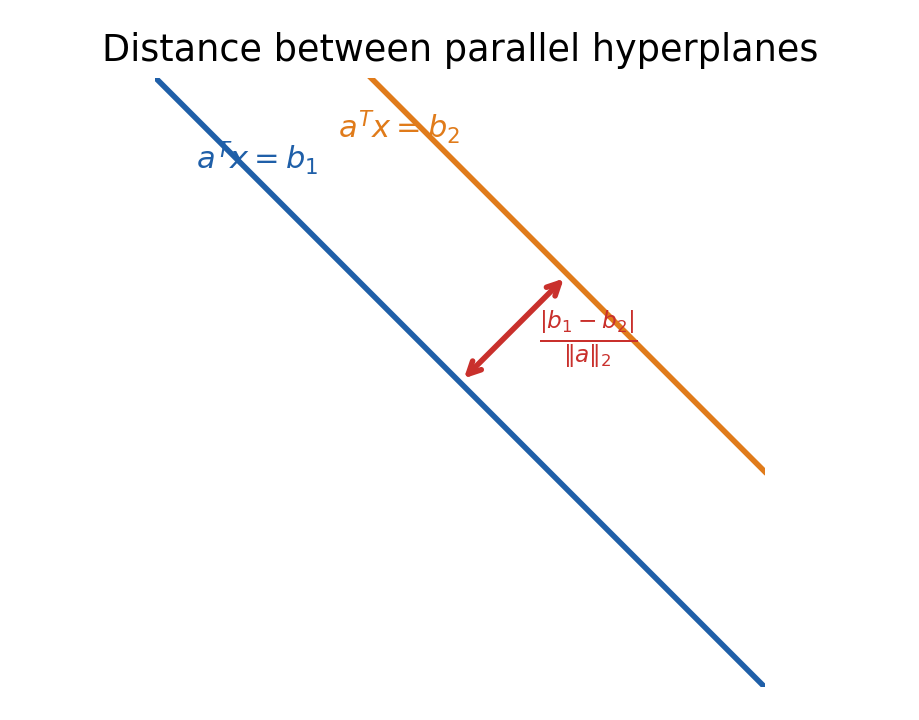
\includegraphics[width=.32\textwidth]{figures/parallel_hyperplanes.png}
\caption{The gap between parallel hyperplanes is measured along the common normal $a$.}\end{figure}

\noindent\emph{Sanity check.} If $a$ is a unit vector, the hyperplanes $a\T x=b_1$ and $a\T x=b_2$ sit at signed offsets $b_1,b_2$ along $a$, so the gap is $|b_1-b_2|$. Rescaling $a\to\alpha a$ (which rescales $b_i\to\alpha b_i$ for the same geometric planes) leaves the formula invariant, as it must.

%======================================================================
\appendix
\section{Code and numerical checks}\label{app:code}

The figures in this document were produced with \texttt{matplotlib} (\texttt{make\_figures.py}). The verification script below was run with NumPy; its output follows.

\lstinputlisting[basicstyle=\ttfamily\footnotesize]{verify.py}

\noindent Output:
\begin{lstlisting}[language={}]
Problem 3: memberships agree on all samples: True (42872 of 100000 points closer to v1)
           midpoint on boundary: c^T m - d = 0.0
Problem 4: 3023 points in set; 0 of 5000 random convex combinations left the set
\end{lstlisting}

\end{document}
